
\documentclass{cmspaper}
\usepackage{xspace}
\usepackage{verbatim}

% The graphics extensions below support using pdflatex to make
% pdf files. They say that, if you compile with latex, the graphics
% package should look for file.eps but that if you compile with
% pdflatex, the graphics package should look for file.pdf or other.
%\usepackage{ifpdf}
%\ifpdf
%  \DeclareGraphicsExtensions{.pdf,.png,.jpg,.nps}
%\else
  \DeclareGraphicsExtensions{.eps}
%\fi

% Code inline with text
\newcommand{\code}[1]{\texttt{#1}}
% Code in its own quotation. Needs \usepackage{verbatim}.
\newenvironment{codequote}{\hfill\minipage{0.9\textwidth}\small\verbatim}%
{\endverbatim\endminipage\hfill\par}

% Macros for usage narratives
\newcounter{countnarrative}
\renewcommand{\thecountnarrative}{N\arabic{countnarrative}}

\newenvironment{narrative}[1]{\medskip\par\noindent\refstepcounter{countnarrative}%
\textbf{\thecountnarrative. {#1}}\par}{}

\begin{document}

%==============================================================================
% title page for few authors

\begin{titlepage}

% select one of the following and type in the proper number:
%   \cmsnote{2005/000}
  \internalnote{2006/000}
%  \conferencereport{2005/000}
   \date{5 September, 2006}

  \title{A 2006-07 Roadmap for CMS Dataset Bookkeeping System}

  \begin{Authlist}
  Anzar Afaq,  Lothar Bauerdick, Stefano Belforte, Andrew Dolgert, Peter Elmer, Alessandra Fanfani, Ian Fisk,  Chris Jones,  Valentin Kuznetsov,  Stefano Lacaprara, Lee Lueking, Dan Riley, Vijay Sekhri, Elizabeth Sexton-Kennedy     
\Instfoot{fnal}{FNAL, Batavia, IL, USA}
\Instfoot{italy}{Italy}
\Instfoot{cornell}{Cornell, Ithaca, NY, USA}
\Instfoot{Princeton}{Princeton, Princeton, NJ, USA}
\Instfoot{balonia}{Balonia, Balonia, Italy}
  \end{Authlist}

% if needed, use the following:
%\collaboration{Flying Saucers Investigation Group}
%\collaboration{CMS collaboration}

%  \Anotfoot{a}{On leave from prison}
%  \Anotfoot{b}{Now at the Moon}

  \begin{abstract}
    Based on the discussion and material presented at the DBS Workshop held at Cornell, this is a roadmap for the concepts and development of the CMS Dataset Bookkeeping System (DBS). The workshop brought together data management, work-flow management, CMSSW framework and other CMS areas, to discuss, document and devise a work plan for DBS that will be followed for the next 6 months. This will provide the needed function and features for the testing throughout 2007 and the beginning of data taking in Fall of 2007.
 
  \end{abstract} 
  
\end{titlepage}

\setcounter{page}{2}%JPP


%
%==============================================================================

\section{Introduction}

The DBS Workshop held at Cornell July 20-22 of 2006 brought together 18 people experienced in many areas of CMS software and Computing to discuss the uses and plan for the CMS  Dataset Bookkeeping System. The DBS project has developed over the last year  a prototype architecture,  schema and API that is sufficient for the CSA06 challenge work, but insufficient to meet CMS's long-term needs. Our mission was to bring together experts in data management, work-flow management, CMSSW framework and other CMS areas, to discuss, document and devise a work plan for the dataset bookkeeping system to  follow for the next 6 months. The system discussed will provide the needed function and features for the testing throughout 2007 and the beginning of data taking in Fall of 2007. This document establishes the overall vision, requirements, and scope for the project, and begins to work out implementation details and a work plan.

\section{DBS Workshop Overview}

\subsection{Goals for Cornell workshop}

Workshop Goals:
\begin{enumerate}
\item Agree to a set of common definitions used in describing the DBS system. Deliverable: Glossary document.
\item  Produce a set of use cases we think are representative of the needs of CMS analysis in general, but targeting the DBS specifically. Deliverable: Documented use cases and work user flow diagrams illustrating them.
\item  Explore existing data management and discovery systems employed by HEP experiments and identify features we would like to have for CMS. Deliverable: Document describing key features we may have overlooked in CMS.
\item  Understand the needed relationships between DBS and the other components of DM and WM systems. Deliverable: Concept diagram showing the relationships.
\item  Understand the relationships between DBS and the CMSSW Framework. Deliverables: Document describing this and diagrams as needed.
\item  Understand the relationships between DBS and the many other sources of non-event information in CMS such as trigger, luminosity, run configuration, run quality information, calibration, alignment, ... Deliverables: Concept map showing the relationships.
\item  Understand how DBS will fit into the picture for the various tiers of CMS computing such as, online, Tier 0, Tier 1, Tier 2 and Tier-n. Deliverable: Document the specific and overlapping needs for each tier.
\item  Establish a set of written requirements for the DBS. Deliverable: Document
\item  Review the existing CMS DBS system, its schema and API
\item  Devise (revise) the schema and API to meet the requirements. Deliverable: Updated schema and APIs. Revise existing DBS description document.
\item  Update the design for the overall DBS system, servers, clients, et cetera. Deliverable: Description document and diagrams.
\item  Explore options for data discovery desirables, and techniques for doing them. Deliverable: Document and list of things to try out.
\item  Discuss possible implementation options. Prototype if time permits. Document issues and further work needed to make final choices. Deliverable: Description of options and motivation for any particular choices. Description of additional work needed.
\item  Draft a plan, describe deliverables, estimate work, prioritize, schedule and assign tasks. Deliverable: Description, schedule, assignments, milestone dates.
\end{enumerate}

\subsection{Workshop Topics}

\begin{itemize}
\item Review of existing DBS system
\item Glossary of terms
\item Use cases for Data analysis
\item EDM/FW connections to DBS 
\item DBS In the context of DM and WM
\item A look at CLEO, Run II, and BaBaR approaches
\item DLS Interactions with DBS 
\item CRAB Interactions with DBS
\item Monte Carlo Request system present and future 
\item Additional DBS Scenarios 
\item Details of and alternatives to existing prototype 
\item Data discovery needs and approaches
\end{itemize}

\section{Glossary and Concepts} 
\subsection{Glossary}
\begin{description}
\item{Dataset}-"any set of 'event collections' that would naturally be
grouped and analyzed together as determined by
physics attributes" -ctdr
e.g., common trigger path or MC generator (configuration?)
e.g., "a particular object model representation of those events" such as
RAW, RECO, AOD??
\item{Primary Dataset}-"data at all levels of processing pertaining to a given
trigger or common MC production criteria" -dm-dbsv0.85
"For Monte Carlo data 'primary datasets' comprise
data generated with the same parameters" -dm-dbsv0.85
Is the set of MC primary datasets bounded? Determinable?
\item{Processed Dataset}- "a slice of data from a Primary Dataset defined by the
processing history applied to it" -dm-dbs-v0.85
"will correspond to a large production of data with a
single major software release version, but may include
multiple minor versions for small bug fixes and also
may contain the output of multiple processings of
some given input event collection" -dm-dbs-v0.85
��multiple minor versions lost in some versions of the DBS schema
\item{Analysis Dataset}- "A subset of Event Collections from a given Processed
Dataset" -dm-dbs-v0.85
Adds constraints to processed dataset
Similar to CLEO EventStore ��physics grade--the data physicists should run
on?
Gone from current schema, no mechanism to create one
\item{Data Tier}- "2.5.1 Data Tiers" -ctdr
DAQ-RAW, RAW, RECO, AOD, TAG, FEVT
"type of content resulting from a degree of processing
applied to the data" -dm-dbs-v0.85
What about RECO and AOD?
Actually defined by the objects contained?
Then data tier is an attribute of a file or event collection, not processing?
What about data tier evolution? AOD2, AOD3, ...?
Or finer grained processing path (not in framework provenance)?
\item{Event Collection}-The smallest unit that a user is able to select through
the dataset bookkeeping system" -ctdr
e.g., event data from a particular trigger selection from one given run
"a single event collection will give access to data from
exactly one data tier" -dm-dbs-v0.85
Currently supporting multiple data tiers, e.g., FEVT
Relationship to file one-to-many or many-to-many
many-to-many for old EDM?
\item{File Block}- "a set of files likely to be accessed together" -dm-dbsv0.85
data management packaging unit
"will in general correspond to the same Primary
Dataset, Data Tier and Processed Dataset" -dm-dbsv0.85
incorrectly reflected in schema?
\item{non-event data-Non-event data}: detector configuration, conditions, ...
Mostly time domain: run, luminosity interval?
DBS currently knows nothing about this
so we told Drew not to work on them
Is this in scope for DBS? If not, what should answer these queries?
\end{description}
(Add additional list to appendix of general ``domain'' terms that Drew/Dave Dykstra have)
\subsection{Concepts in more detail}
\subsubsection{Analysis Dataset}

(Assignment: Dan will fill this in)

\section{DBS interaction with other DM, WM areas, and CMS at large}
The role of DBS in CMS as described in the Computing TDR~\cite{CTDR}.

(Assignment: Drew - Broad overview of DBS form Pete's talk.Workflow tools are interoperable through using the DBS API. ) 
\subsection{DLS}

(Assignment: Alessandra to fill this in)

The Data Location Service (DLS) provides the means to locate replicas of data in the distributed computing system. 
It maps file-blocks to storage elements (SEs). It
provides only the  names of sites hosting the data and not the physical location of the constituent files at the sites. The attributes for data in DLS include  (custodial  replica = considered a  permanent copy at a site)

 Interactions with DLS include 
\begin{enumerate}
\item Insert file-blocks produced at a site (MC Production)
\item Insert file-blocks upon data replication (PhEDEx)
\item Query to locate file-blocks (CRAB, MC Production)
\end{enumerate}



Fileblock name
DBS knows how dataset are organized in term of fileblocks
DLS knows fileblocks locations
 Fileblock name needs to be consistent across DBS and DLS
Local scopes DBS/DLS upload into global DBS/DLS (clashes on fileblock name?)
Data discovery and location: combine DBS and DLS information.



\subsection{PhEDEx}
Assignment: Lee Ref to PhEDEx. Ask Lassi for text.)
\subsection{DBS Context Diagram}
The DBS system is just one component in the Data Management system, and also has relationships to other sources of information in CMS at large. An overall picture of CMS is illustrated in Fig.~\ref{fig:dbs-context-diagram} with DBS represented in the center. 

\begin{figure}[hbtp]
  \begin{center}
    \resizebox{15cm}{!}{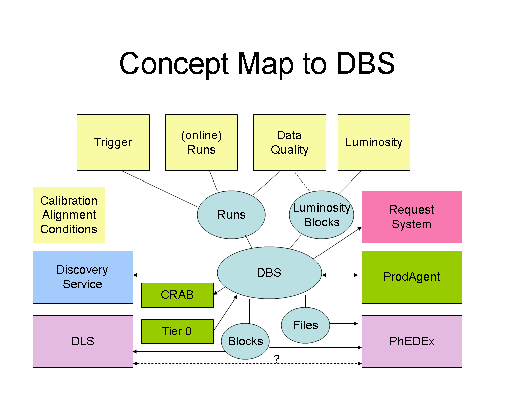
\includegraphics{figure/DBS-WS-DatabasesConceptMap-20060721.eps}}
    \caption{Concept diagram for DBS within CMS.}
    \label{fig:dbs-context-diagram}
  \end{center}
\end{figure} 

(Assignment: Lee will fill this in)

\section{Tasks and Use Cases from the  Workshop}

During the Cornell Workshop we compiled a list of 51 items to be followed up in our work to design the DBS system. There are several categories for the items and we have characterized them here as 1) use cases to be further expanded, 2) design requirement, 3) relationship with other subsystem in Data Management, 4) relationship within CMS at large.

\subsection{ Use cases to be further expanded}

   1.  (Assignment: Vijay)(use case, fermilab)Need to develop use case for publishing locally analyzed data to global scope - Fermilab

   2. (Assignment: Dan)(dbs)Fix a subset of a dataset due to problem found later, e.g. sqrt (-1) (changing does not affect the physics when it does not happen), calibration change. These are cases where only selected parts of the data need to be reprocessed, and then "blended" back in to the data set"

   3. (Assignment: Dan)(dbs)Need to track event processing failures in dbs, as reported by EDM in the job report run, event, reason for failure.

   4. (Assignment: Dan)(dbs)use pass ID to determine what data is interesting to analyze. Pass ID is equivalent to processing path name.

   5. (Assignment: Dan)(dbs)Allow for fruit salad mixing of data in a processed dataset.

   6. (dbs)Store filter information for each file (stream) for multi-output skimming


  14.(Assignment: Anzar) (dbs) Users need to store special data, such as log files or personal or group data.


  17. (review w/ ProdAgent, dbs)Merge and remapping requirements and use case. Is it really required (or advisable) that we get rid of intermediate files? Refer to SAM experience reported by Adam.

  19. (dbs)Who or which group created a particular set of data?

  21. (dbs, in progress)Schema review items: does family have any meaning in CMS? , Dans talk, review SAM schema, others.

  22. (use case-Drew,Lothar)Additions needed for CSA06: 1. find data based on application version, 2. link with DLS to find where data is.

  23. (use case) Need to go through analysis workflow (use cases) and determine additional API calls that will be needed.

  24. (Assignment: Dan)(use case-C.Jones)How is Analysis data set defined and how will it be used? Will it be static or dynamic (changes as new data is added or old removed)? Is there something like a snapshot? Are names prescribed for Anal DS, are they pre-fabed by physics groups or other admin policy. Can users create their own at will? What will UI look like, what is API required.?

  25. (dbs, FJR)Need way to have the set of tags (one for each subsystem) specifying calibration and alignment into DBS so it can be query-able. (it is in the config file)

  26. (Assignment: Anzar)(dbs) Introducing data from out side official processing machinery, so-called offroad data"

  27. (Assignment: Anzar)(usecase-?)Private and semi-private data sharing. How can you share data with colleagues at other institutions before it is ready for global scope publication.

  28. (Assignment: Lee)(dbs)Getting runs into DBS, need DBS to have relation to luminosity block information.


  32. (dbs,FJR) Data tier is defined well enough to know what objects are in it. Some concern that this will change. How can we store the branch information from the FJR in a useful way? How will it be queried?

  33. (dbs) it is not correct to define parentage between processed datasets as some child data may be missing. Better to define at the file level.

  34. (dbs, some assumptions to clear up)Need way to select individual events from a particular tier given run/event.


  37. (dbs,FJR)The FJR should contain as much as possible of the information that is recorded in DBS.


  42. (?) Explore use of defaults for data specification [e.g. do not make people say 'AOD' since that is the most requested]

  43. (need more inout)How is DBS used for Online? what might DBS Track?
         1. Laser data
         2. alignment stuff
         3. express stream
         4. dedicated calibration runs
         5. Physics data> ==> Does DBS begin before or after repacking? << big issue. 


  44. (Assignment: Drew) (use case) How is DBS used for Tier 0?
         1. Reconstruction
         2. Tracking calibration and alignment output data 

  45. (Assignment: Drew)(use case) How is DBS used in Tier1:
         1. Re-reconstruction
         2. skimming 

  46. (Assignment: Drew)(use case) How is DBS used in Tier 2?
         1. MC Production
         2. Data analysis 

  47. (Assignment: Anzar)(usecase) How might DBS be employed for MTCC and Test Beam data?
         1. If a run table is added thenthis type of data could be added
         2. Under no pressure to make this work on a short time scale, but can use run for existing data to load the DBS catalog.
         3. Would be useful experience for the DBS system and good interaction form physicists. 

  
50. {Assignment: Valentin, in section on data discovery)(use cases) Data Discovery use cases and what should be available for discovery (Need subgroup to further explore this):
         1. detector experts looking at detector problems, Range of data (run range) with certain conditions, bad detector component, special trigger.
         2. What Physics meta data is needed to be related to datasets? Is it good enough to have 'simple' trigger name or all details of trigger needed? What high-level query-able things needed to store to find data? We need to make 'synthesized' easy to query versions AND allow full physics physics metadata discovery. 

  51. (dbs) From schema discussion:
         1. Three main concepts (more when have pictures of notes):
               1. Files
               2. Processings
               3. Datasets 
         2. We see no need to continue the concept of event collections.
         3. Schema was discussed and sketched out at workshop. Anzar will enter and draw using druid. 


\subsection{Design requirement}

  10. (dbs)All copies of a physical file are lost. Must be able to mark the status as unavailable or lost. Needs to be reported to DLS, and PhEDEx also.
  15. (Requirement)(dbs)Group needs a way to specify "official" data sets or analysis datasets.

  16. (Requirement)(dbs)Primary datasets must be special and have special meta data or ability to link to other information that characterizes it.


  18. (Requirement)(dbs)Authentication and authorization for DBS API

 new. Status flags for files, whatelse?

\subsection{Relationship with other subsystem in Technical Project}
   7. (dbs, need more info)support for pileup input datasets/files.

  11. (ReqSys?)Need a way to specify and submit processing requests for MC generation, and general data processing.

  12. (ProdAgent)Recovery of files that were not processed due to input failures, or high error rates in application.

  13. (ProdAgent)Recovery of data lost after processed. Outfile is lost 1. before entered into DBS, or 2. after entered in DBS.

  20. (?)Naming convention for processed dataset. Can this be automated.


\subsection{Relationship within CMS at large}
   8. (use case-?)data quality information. What level of granularity? run, luminosity block, event?

   9. (dbs, use case-?)Must be able to track luminosity for analysis dataset. Run over N luminosity blocks, some fail, some pass. How to integrate luminosity for all data used.

  29. (?)Need to have LFN naming convention.

  30. (use case, need more input) High level trigger information in DBS based on trigger mask, or trigger object, so can discover data based on trigger.

  31. (use case, need more input)Luminosity information stored in DBS? This information may change with time. Could have lumi block ranges and get luminosity from lumi DB.


  35. (ProdAgent, dbs, Valentin)Need way to track, monitor, record usage patterns of the data access. Way to study history of data access. 

Here are the contact points between ProdAgent and DBS:
\begin{enumerate}
\item DBSComponent
\begin{itemize}
\item Creates Datasets   (both merge and processing)
\item Populates Datasets  (both merge and processing)
\end{itemize}

\item MergeSensor
\begin{itemize}
\item  Watches Datasets in polling mode
\item Retrieves fileblock information, generates merge jobs when sufficient data is present
\end{itemize}

\item PhEDExComponent
\begin{itemize}
\item  Queries DBS for fileblocks for an entire dataset for PhEDEx injection
\end{itemize}

\end{enumerate}


Other uses (not yet implemented but mostl likely will be)
\begin{itemize}
\item Remap Merge file parents to processing file parents upon completion of a merge job (DBS Component)
\item Validation/Invalidation of files in DBS
\end{itemize}
note: FJR shows which branches were used. probably want to dump FJR and logs in to archive, could be DBS. 

  36. (dbs, need more input) How is file block name handled when published local to global scope DBS. Are files within the file block rearranged. Are more block attributes needed?

  38. (use case-?)What is the software environment an analysis user will be using while in the local scope? Who moves data and DBS info about the data from local to public scope and how is it accomplished? What is the software setup, configuration, and what tools are needed? What authentication and authorization is needed for this?

  39. (ReqSys?-Giulio, dbs-fnal)Use cases for the data processing request system for both MC and real physics data processing. What is the overlap between the request system and DBS? DBS and the Request system share discovery of 'applications' (i.e. the configuration). It is assumed this sharing will not be needed for CSA06 but should be understood for the final system.

  40. (ReqSys?-Giulio) Confusion about meaning of payload and workflow in MC request system [Guillio needs to make a glossary that synchs up with the DBS jargon].

  41. (ReqSys?, dbs Gulio,Pete,Lee)The Request System and DBS are related but Peter thinks should be 'decoupled'. It seems possible and useful to link up the parameter set discovery system of the two in the long term. Not needed for CSA06.

  48. (Assignment: Ian) (use case, dbs?) DBS/DLS/PheDex know about file/file block sizes
         1. How is this space 'assigned'/'allocated' at Tier-2 sites?
         2. Need tools to determine how disk (resources?) are used by "groups" in CMS?
         3. detail: Need to have concept of ownership (grolup/user) in either DBS or DLS
         4. research: map how people running jobs work within the constraints of the existing system (how do they deal with disk allocations, and stepping on one another's resources?) 

49. (need to present to other cms db players - Lee) Concept map for DBS and how it relates to other event and non-event data repositories. (DLS/DBS, conditions DB, trigger DB, luminosity DB, et cetera.

\section{Use Cases}


\subsection{Use cases for CSA06}

Several use cases for the upcoming CSA06 work are illustrated in Fig.~\ref{fig:csa06-use-cases-diagram} and described in this section. CSA06 will use Monte Carlo data to simulate real data from the detector. This data will pass through the HLT and all production steps, ending in several steps of physics analysis. The CSA06 test will use a version of the DBS and other tools current as of July 2006.
\begin{figure}[hbtp]
  \begin{center}
    \resizebox{0.8\textwidth}{!}{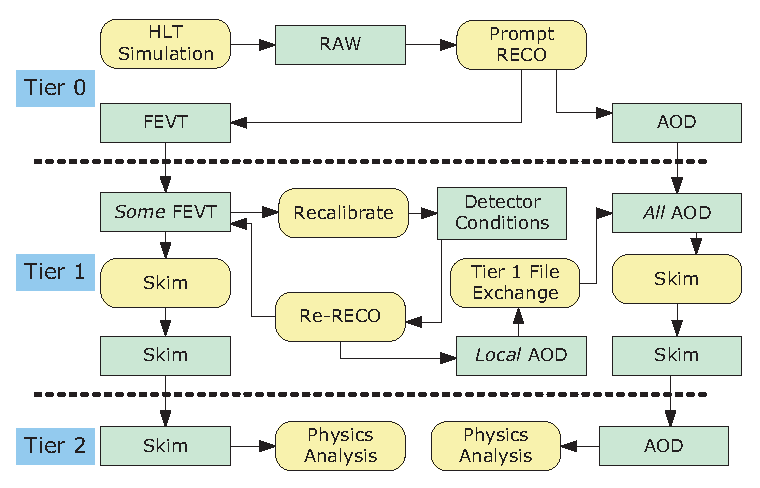
\includegraphics{figure/CSA06_use_cases_dfd.eps}}
    \caption{This data flow diagram for CSA shows processing in yellow
    and products in green. PhEDeX performs transfers across data tiers
    and the ``Tier~1 File Exchange" of AOD among Tier~1 storage.}
    % To make eps from Visio, save as WMF. Open in Illustrator and save eps and pdf.
    % Include fonts. Use Acrobat full version to trim the pdf page.
    \label{fig:csa06-use-cases-diagram}
  \end{center}
\end{figure} 


\begin{narrative}{Production Manager Creates Real HLT Data from MC Data}

Production Manager runs the HLT on a large dataset of MC Data. Production Manager uses Y to put that data into the DBS. Only five million events go through the HLT from all of the MC data, and DBS tracks these.
\end{narrative}

\begin{narrative}{Tony at Tier~0 Presents Raw Data from HLT\label{narr:tony0}}

Tony uses a set of scripts to process simulated HLT data. He asks X to make file blocks from that data. He asks Y to put that data into the DBS. \emph{Actually, I think Tony produces RAW, RECO, FEVT, and AOD at one go, right?\/} Tony gives tool Y a list of information, which we will figure out below. Tool Y contacts the Global DBS to place correct processing history.

What tool is used at the Tier~0 to insert RAW data into the DBS? How are the primary datasets for real data managed at the tier0? How are primary datasets for MC handled?

Data discovery requirements: Management of primary dataset IDs at the Tier~0.
\end{narrative}

\begin{narrative}{PhEDeX Transfers Data Among Facilities\label{narr:phedex}}
All of the places that the diagram shows a transfer, it is done by PhEDeX. Someone tells PhEDeX to look for a particular file in the DBS, and it will transfer that file. How does it identify that file? Is there a set of search criteria, so that any file matching a description is transferred?
\end{narrative}


\begin{narrative}{Alignment Person Recalibrates Using Z to $\mu$-$\mu$ to Produce a New Version of Alignment\label{narr:recalib}}

Data Quality Expert polls a tool which shows a list of available datasets. He knows that he is looking for FEVT from CSA06 and that this FEVT data should be straight from the HLT, not reprocessed in any way. (Should be done at CAF, but not for CSA06.)

He submits the alignment job to CRAB or Prodagent. He specifies a subset of the total FEVT dataset. The recalibration job returns new detector conditions. He gives these detector conditions to \emph{someone\/} who places them into alignment database where they will be found by future RECO production. (It could be a job robot that runs this instead of Prodagent or CRAB. How do you insert new detector conditions? Do you need a new version of the software or configuration.)

The Data Quality Expert then asks Prodagent to create RECO and AOD from the RAW data within the FEVT. He already knows the exact dataset but may use a different subset than was used for recalibration. Prodagent performs this calibration and creates a new, partial set of FEVT and AOD.
\end{narrative}

\begin{narrative}{Physicist Tier~2 Creates Skim of Re-RECO at Tier~1\label{narr:skim2}}

Physicist looks for re-RECO data from a recalibration at Tier~1. (Will there be more than one?)
Finding that dataset, he asks which Tier~1 has that data. He puts some identifier for the dataset into a Prodagent job, along with the name of the Tier~1 on which to do processing. Prodagent creates the skim and registers it in the Global DBS.

Data discovery requirements:
\begin{itemize}
    \item Identify data as CSA06 -- by primary dataset name?
    \item Identify a skim -- by processed dataset name?
    \item Locate a dataset -- /primary/tier/processed $\rightarrow$ blocks $\rightarrow$ SE via DLS 
\end{itemize}
\end{narrative}



\begin{narrative}{Physicist Tier~2 Runs Analysis Job}
Physicist has just created a skim of Tier~1 FEVT data from re-RECO. He needs to tell PhEDeX to transfer that data to his Tier 2 site. Then he tells CRAB to run that job.
\end{narrative}


\begin{narrative}{Physicist Tier~2 Runs Skim on One of Six Copies of AOD}
This is much like narrative~\ref{narr:skim2} except that the file type is AOD. He must perform a skim at a Tier~1, ask PhEDeX to transfer that skim to the Tier~2, and then process it.
\end{narrative}


\begin{narrative}{Production Manager Watches CSA06 Progress}
Production Manager wants to see what data exists and what file blocks are transferred. They open a web page tailored to CSA06. It queries the DBS for file existence and PhEDEx for file transfer rate. (Can PhEDEx tell you this? Would something else do it, like the DLS?)

Data discovery requirements: Identify a subset of CSA06 MC data injected at the HLT (differnet primary dataset?).
\end{narrative}

\subsection{Data Discovery for CSA06}
From the usage narratives above, we can compile needs for data discovery.
\begin{itemize}
\item PhEDeX identifies a subset CSA06 FEVT data for transfer to Tier~1. (\ref{narr:phedex})
\item PhEDeX identifies CSA06 AOD data, whether produced by Tier~0 or Tier~1, and transfers it to particular Tier~1 facilities which subscribe to different trigger lines. (\ref{narr:phedex})
\item PhEDeX identifies a particular skim dataset, created by a Physicist, from Tier~1 to Tier~2. This can be either FEVT or AOD. (\ref{narr:phedex})
\item Data Quality Expert needs CSA06 FEVT data that is identifiable as coming straight from Tier~0. (\ref{narr:recalib})
\item Prodagent has to be able to find RAW data within an FEVT dataset. (\ref{narr:recalib})
\item Physicist must identify re-RECO and find what Tier~1 facility has the data. (\ref{narr:skim2})
\end{itemize}
Given these requirements, what should Tony-at-Tier-0 put into the DBS? Our working trial is the following:
\begin{itemize}
    \item file blocks by LFN,
    \item application name, family, and version for each step, and
    \item data set names, such as \\ \code{/csa06-081-os-minbias/DIGI/CMSSW\_0\_8\_1-GEN-sim-digi-1154005302-merged}, \\ where the primary dataset indicates that this is CSA06.
\end{itemize}
The primary dataset will start with \code{csa06} for this data. Whether it is RAW, FEVT, RECO, or AOD is encoded in the data tier, as was planned. The software version won't help identify re-RECO because it changes the conditions database, not the software version. We could identify re-RECO by changing the processed dataset name, as is done with \code{merged}.

How would we like do data discovery after CSA06? The dataset name encodes the primary dataset and data tier clearly. We would prefer not to use the processed (or analysis) dataset name to encode something a computer needs to understand. What other qualities do computer programs need to identify?
\begin{itemize}
\item When you subscribe to a particular dataset with PhEDeX, it should be able to know that future re-RECO of that dataset, or other reprocessing of that dataset, is associated with the same subscription.
\end{itemize}
I don't see anything else to encode.

\subsection{Use Cases Long-term Project}

\subsubsection{Monte Carlo Production}
\subsubsection{Physics Data Production}
\subsubsection{Data Analysis}

\section{DBS client server Architecture}
\subsection{Requirements}

+ DBS Access What are the avenues through which the DBS information will be accessed?

\subsubsection{Overview of usage}

   1. Production processing
         1. ProdAgent 
   2. Group processing
   3. Individual processing
   4. Individual and group analysis
         1. CMSSW
         2. ROOT
         3. Other tools, shells, et cetera 
   5. Interactions and relationships with other CMS databases
         1. Trigger, Luminosity
         2. Online Runs
         3. Conditions, et cetera. 

\subsubsection{Access}

   1. API
         1. CRAB
         2. ProdAgent
         3. Framework (CMSSW) through some wrappers?
         4. ROOT ?
         5. Primary language is expected to be Python, but could include C++, Java, et cetera. 
   2. Command Line Input
         1. Designed to work conveniently with standard Unix commands
         2. based on API 
   3. Web tools
         1. Initial tools will use API
         2. May grow beyond API
         3. Include high level search and discovery features 

\subsection{Options for service architecture technology approaches}
There are at least two issues here, 1. server technology, and 2. transport and messaging layer. The two can be closely related as the tools provided for the messaging layer are better for some server solutions than others.
Server options

\begin{enumerate}
\item  CGI/Perl: Continue to develop CGI w/ Perl scripts
\item  CGI/Python: Continue to use CGI, but rewrite scripts in Python
\item  Servlets: Use Tomcat servlet container and implement API in Java servelets.
\item  Commercial Appserver: Use a commercial application server solution, for example JBOSS and Hibernate.
\item  C++ DBS AppSrv?: Reuse the DBS App server developed at FNAL under a standard server technology, like Apache, or Tomcat.
\item  RAD or Agile Web technology: Use one of the recent rapid web development platforms, for example Ruby On Rails (Ruby), or Django (Python), Zope 3. 
\end{enumerate}
Transport and messaging layer
\begin{enumerate}
 \item  Assume the transport layer is HTTP
 \item  Messaging layer can have a couple of choices
         1. Standard like SOAP, XML-RPC, REST
         2. We make something that is performant (like the XML messages used now for CGI, or something similar to Frontier). 
\end{enumerate}
\subsubsection{Criteria for decision}
\begin{enumerate}
 \item  Must be proven technology
 \item  Not out dated
 \item  Well supported by existing tools and documentation
 \item  Flexible framework that we can grow to meet future needs
 \item  Provide needed scalability
 \item  Easily maintainable
 \item  Accommodate schema evolution
 \item  Accommodate API evolution
 \item  Server functions must be well factor-able
 \item  Provide "local" and "global" scope functionality. This implies a. using multiple database technologies and a. having access through local library or remote server.
 \item  Meet performance needs. This depends on transport and messaging layer employed.
\item   Web Services support. This is a desirable, and determines the flexibility for the future. 
\end{enumerate}



Decision matrix can be found in Table~\ref{tab:tech-options}.
\begin{table}[htb]
    \caption{Features provided by each technology option. X=Yes,*=Maybe, but involves more work, ?=Unknown, or too soon to tell, Blank=No  }
    \label{tab:tech-options}
    \begin{center}
      \begin{tabular}{|l|c|c|c|c|c|c|} \hline 
Criteria/Approach & CGI/Perl & CGI/Python & Tomcat w/ Java &C++ App & Jboss &Ruby\\
                  & (CSA06)  &            & Servlets      &Hibernate & Server& on Rails \\ \hline
 Proven           & X & X & X & X & &      \\
 Modern           &   &   & X & X & &    X  \\
 Supported        & X & X & X & X & &    ?  \\
 Flexible         &   &   & X & X & &   ? \\
 Scalable         & X & X & X & X & & ?    \\
 Maintainable     & * & X & X & X & &   ?  \\
 Schema evolution & * & * & X & X & X &   ?  \\
 API evolution    & * & * & X & X & X &  ?  \\
 Easily factorized& * & * & X & X & X &  ?  \\
 Mult DB backends &   &   & X & X & X &   ?  \\
 Accessed via lib 
     or server    & X & X & X & X & X &   ? \\
 Performance      & X & ? & X & X &   &*       \\
 WS Support       &   &   & X & X & * & ?       \\ \hline
      \end{tabular}
    \end{center}
  \end{table}  
%put into tablualr format
%\begin{verbatim}
%Criteria\Approach 	CGI/Perl 	CGI/Python 	Java Servlets/tomcat 	JBOSS/Hibernate 	C++ DBS AppSrv? 	RUBY on Rails
%1. Proven technology 	X 	X 	X 	X 	  	 
%2. Not out dated 	  	  	X 	X 	  	X
%3. Well supported 	X 	X 	X 	X 	  	?
%4. Flexible framework 	  	  	X 	X 	  	?
%5. Scalability 	X 	X 	X 	X 	X 	?
%6. Maintainable 	* 	X 	X 	X 	  	?
%7. Schema evolution 	* 	* 	X 	X 	X 	?
%8. API evolution 	* 	* 	X 	X 	X 	?
%9. Well factorized 	* 	* 	X 	X 	X 	?
%10a. Mult DB backends 	  	  	X 	X 	X 	 
%10b. Access via lib or server 	X 	X 	X 	X 	X 	 
%11. Performance 	X 	* 	X 	X 	* 	?
%12. WS Support 	  	  	X 	X 	* 	?

%    * X=Yes
%    * *=Maybe, but involves more work.
%    * ?=Unknown, or too soon to tell
%    * Blank=No 
%\end{verbatim}

\section{Data discovery needs and options}

\subsection{Needs for Data Discovery}

\subsubsection{Data discovery}

 need a clear definition of ��data��
 who are the actors
 versioning
 level of granularity
 push or pull model
 data, meta-data, luminosity ....
 descriptive criteria

\subsubsection{Data discovery prototype}
The current DBS Data Discovery prototype has been shown on Figure \ref{fig:dbs-data-discovery}.
\begin{figure}[hbtp]
  \begin{center}
    \resizebox{10cm}{!}{\includegraphics{figure/DBSDataDiscoveryLayers.eps}}
    \caption{DBS Data Discovery prototype.}
    \label{fig:dbs-data-discovery}
  \end{center}
\end{figure} 
It based on three external third party packages:
\begin{itemize}
\item {\it CherryPy}~\cite{CherryPy} is the a pythonic, object-oriented HTTP framework.
It has been used as a simple web server for DBS data discovery proptotype.
\item {\it Cheetah}~\cite{Cheetah} is the template engine and code generation tool, 
written in Python. It can be used standalone or combined with other tools and frameworks. 

\item {\it SQLAlchemy}~\cite{SQLAlchemy} is the Python SQL toolkit and Object Relational 
Mapper that gives application developers the full power and flexibility of SQL. 
It provides a full suite of well known enterprise-level persistence patterns, 
designed for efficient and high-performing database access, adapted into a simple and 
Pythonic domain language. It works with well-known DBs, including: ORACLE, MySQL, Postgres, SQLite, 
etc.
\end{itemize}

The multi-tier architecture of the server will allow the usage different type of technologies, e.g.
SQLAlchemy can be replaced with generic Database accesing layer, such as JDBC or Database
connection pool management, CherryPy with apache web server, etc.~\cite{frontier}.

We try to explore the way how physicists will discover new data within CMS experiment. First,
we see clear division between our actors. They are:
\begin{itemize}
\item {\bf physicists} -- this category includes people whose interests extend to identify
data avaialable for analysis, e.g. find Higgs sample which pass certain criterias.
\item {\bf production managers} -- this is a list of actors who are mostly interested in
data production and deployment.
\item {\bf site administrators} -- this category of users are interested in monitoring site
resources, such as disk usage.
\item ...
\end{itemize}

In current prototype we mostly address the CSA06 use casses, the {\bf production manager's} 
point of view to discover data. We start from identifying file blocks based on three 
main search categories:
\begin{itemize}
\item application -- identifies details of software used for data production, e.g. 
CMSSW\_0\_8\_1, as well as the production step, {\it family}, e.g. RECO, and 
name of the executable, e.g. cmsRun.
\item primary dataset -- identifies primary dataset, e.g. CSA06-081-os-minbias.;
\item data tier -- identifies data tier, e.g. RECO.
\end{itemize}
The presentation layer, auto-generated using Cheetah~\cite{Cheetah} templates, represents
the {\bf physicists} and {\bf experts} (such as {\bf production managers} output.
Their difference lies in fine-grained details of data, for instance pn {\bf expert} page
the block/file statuses are shown, while {\bf physicists} output hides such detail and shows
only valid samples useful for generic analysis.

The following extensions are quite visible to implement:
\begin{itemize}
\item list of avialable sites together with details of data on those sites, e.g. for site A we 
summarize the total disk usage, location of files, etc.
\item list of run/lumi-sections
\item list of avaialble datasets with full description of them, e.g.
electron -- electron trigger signal
\item list of applications with full description about their configurations, etc., e.g.
CMSSW\_0\_8\_1 version which includes the following list of config files
\item form which will allow to find parentage information about particular dataset
\end{itemize}

The long term plan may includes development of user-freidnly queriable language for 
data discovery.
\subsubsection{Data to discover}

 we need to discover at least the following items:
 files, file blocks, event collections, runs, datasets,
meta data, data types (e.g. MC/reco)
 But actors have different vision for data discovery:
 Production interested in: files, file blocks, event
collections, data type
 Physicists interested in: event collections, datasets,
runs, meta-data, data type
 data managers/site admins: files


\subsubsection{Meta data}

 Which kind of meta data physicists wants:
 run, dataset, trigger stream, energy, ...
 how they want to express their requests
 who is going to generate meta data
 how meta data will be populated to DBS?
 where meta data will be stored

\subsubsection{Actors behavior}
 we need clear understanding how different actors
behave
 Physicist wants to perform manual discovery at initial step
of analysis and automate the process later
 Phedex will/should perform auto discovery
 site admins/data managers will do it periodically and make it
semi-automatic
 we need a set of tools to support such behavior

\subsubsection{Data indexing}
 All actors mostly interested in fast data access
 DB vs file based indexing
 data indexing level: file block, files, evcoll, ...

\subsection{Possible tools for indexing}
We need to be able to provide search capabilities on the data that most interests analysis use-cases. 
The important parts of bits are in Parameter-Sets that describe how datasets/files are produced.

What we have today in DBS is just a place holder and no real use.
We need to define how we want to store Parameters-Sets in DBS and keep in mind that they are easily search-able.
We can individually add and describe parameter-set(s) into DBS (for example).
This is Pre-requisite to search and discovery, if we don��t have parameters-sets organized somewhere we can��t index/search them too.

Many interesting ideas/tools exists out in the wild, we need to define the Requirements. 
I say we need to index the parameter-sets and some ��other�� characteristics of datasets to make them search-able. We might need to create some definitions and mappings too.
Names that comes to mind a Google, LXR, Apache Lucene���.
We need something that doesn��t return 10,000��� pages (google type searches are out), that, specific to our needs could be tailored (Lucene is in), be capable of searching for specific keywords that makes sense to users but are not actually in the files (LXR is out!). [Sort of maps between what files hold and what it means].


http://lucene.apache.org/java/docs/index.html
Lucene is Doug Cutting's wife's middle name, and her maternal grandmother's first name !. 
Apache Lucene is a high-performance, full-featured text search engine library written entirely in Java. It is a technology suitable for nearly any application that requires full-text search, especially cross-platform. 
open source project 
Lucene is 100% pure Java and has no external dependencies. 
Provides serach and indexing capability, one can write his/her own indexing mechanism and rest is taken care off.

Indexing
over 20MB/minute on Pentium M 1.5GHz
small RAM requirements -- only 1MB heap 
incremental indexing as fast as batch indexing 
index size roughly 20-30% the size of text indexed 

Searching
ranked searching -- best results returned first 
many powerful query types: phrase queries, wildcard queries, proximity queries, range queries and more 
fielded searching (e.g., title, author, contents) 
date-range searching 
sorting by any field 
multiple-index searching with merged results 
allows simultaneous update and searching 

This is shown in  Fig.~\ref{fig:dbs-indexing} and described in this section.
\begin{figure}[hbtp]
  \begin{center}
    \resizebox{15cm}{!}{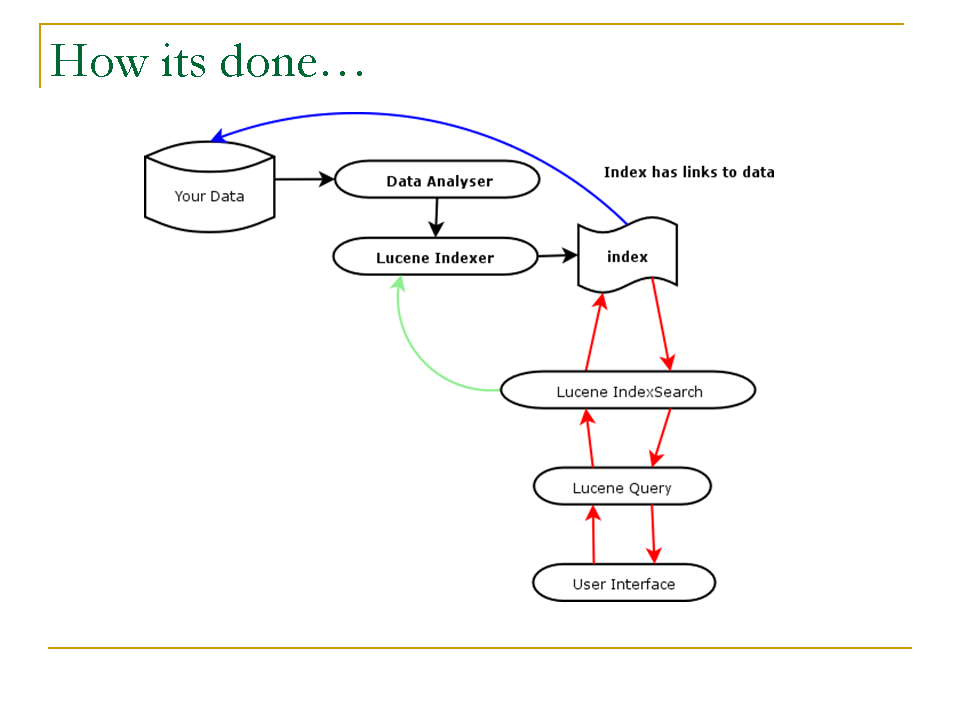
\includegraphics{figure/DBS_Indexing.eps}}
    \caption{Using a tool, such as Apache Lucene, to index parameter files.}
    \label{fig:dbs-indexing}
  \end{center}
\end{figure} 




\section{Framework needs}


This is shown in  Fig.~\ref{fig:framework-access} and described in this section.
\begin{figure}[hbtp]
  \begin{center}
    \resizebox{15cm}{!}{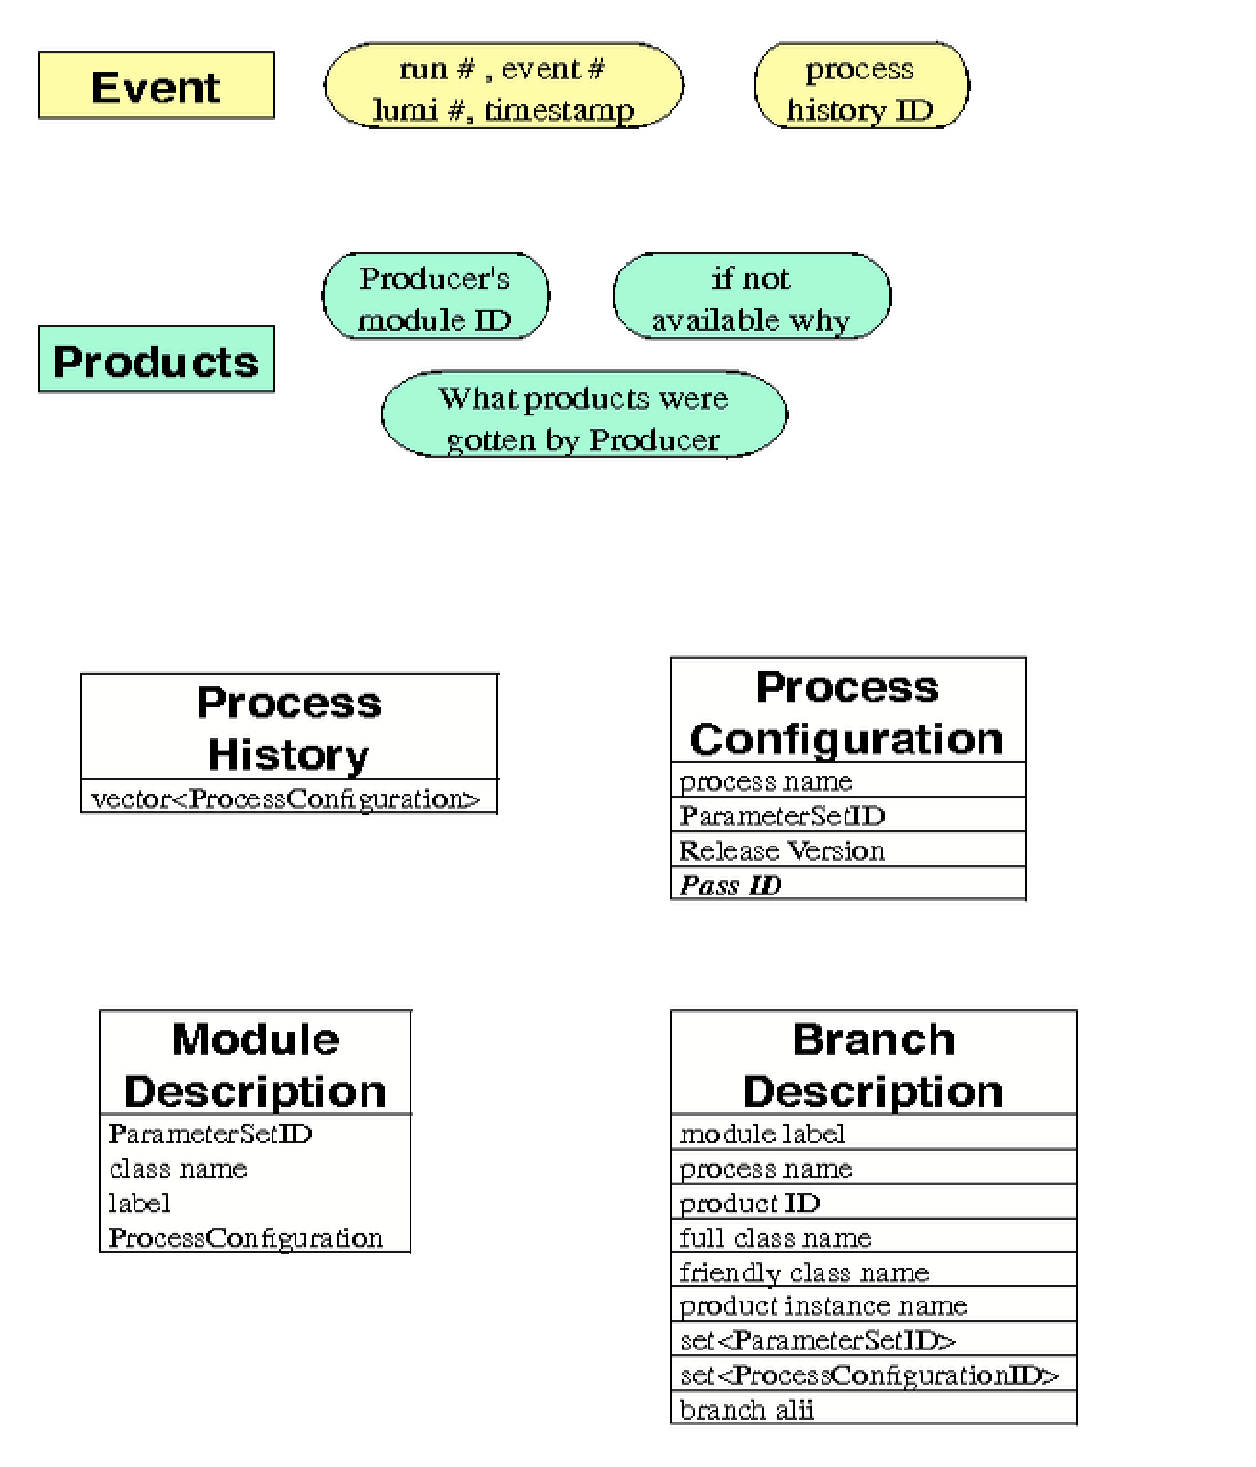
\includegraphics{figure/access.eps}}
    \caption{CMSSW Framework access.}
    \label{fig:framework-access}
  \end{center}
\end{figure} 

\subsection{CMSSW Framework provenance/DBS interaction}

The "Unambiguous identification of reconstruction results" section of the "CMS Core Software Re-engineering Roadmap" is mostly correct (a few things are not implemented yet, and some recent design decisions are not reflected there yet). This page provides a brief summary of the the aspects of the framework provenance which may have implications for the DBS provenance database.

\subsubsection{Framework provenance summary}

There are two kinds of provenance produced by the framework: (1) module configuration for the process; (2) event-by-event, for each object produced, what event objects were accessed by the module producing that object. Event-by-event provenance is dropped if the objects are dropped (TODO: verify); module configuration is always stored (it was decided that garbage-collecting unreferenced configurations was not worth the effort) (TODO: verify). Dropping the event-by-event provenance can lose processing history, since only direct parentage is kept (TODO; verify), but the sequence of processing steps is stored. The module configuration stored is currently the configuration for the entire process (i.e. the union of all the module configurations) (TODO: verify), not a module-by-module configuration, but the module by module configuration can be recovered from the overall process configuration. Provenance tracking for the EventSetup is planned, but not (as of May 2006) implemented yet. The full provenance is written to the output file.

Names/paths of files containing event data are untracked parameters, so they are not recorded in the provenance. There are also no file unique identifiers--the framework, except for the input and output modules, deals with events as objects with no association with any file. Filenames of some conditions data are tracked parameters.

Each CMSSW production process has a "job configuration" name. The job configuration name is a component of the branch name for objects produced in that job, so branch names will be different for objects where the processing steps differ (e.g., SIM/DIGI/RECO in one job vs. three separate jobs). The framework partially hides this, but it is visible in ROOT, so there is a strong incentive to use an identical sequence of processing steps for all objects of a given type. As of May 2006, there are proposals for aliasing branch names which may change this consideration if every branch has an explicitly configured alias.

EDM fast merge will, in one job, only process files with identical provenance. Prior to the 0.8.0 release, the CMSSW Framework had the same restriction. Starting with 0.8.0, CMSSW plans to support "fruit salad" processing, where files with different provenance may be processed in the same job if the provenances are compatible. Provenances are considered compatible if the object name to number mappings are the same for all objects in common between the files. The fast merge does not modify any objects, and does not create any provenance--so far as CMSSW is concerned, fastmerge is completely transparent.

\subsubsection{DBS implications}

At the file level of the DBS, the CMSSW provenance mostly provides constraints. File parentage must be tracked entirely by the DBS--CMSSW does not track it. CMSSW provenance provides a processing history at the object level, not the file level, and the object history may not be a complete record of the processing steps that produced the file containing that object if intermediate objects have been dropped from the output.

The framework allows objects of the same type but different provenance if they differ in the process name, process instance label, or module label. The framework provenance may also include module configurations for objects which are not in the output file, since module configurations are not "garbage collected". The presence of multiple configurations for the same module--for objects which may not even be in the corresponding files--will limit the accuracy and reliability of queries on any "file level" provenance summary. A simple example of this would be if the HLT places reconstructed objects in the output stream which are also produced in prompt RECO or re-reconstruction. At the very least, this would mean that any query on the DBS provenance must include the process name as part of the query, and that may not be sufficient for the analysis use cases envisioned.

\subsubsection{Notes and links}

    * How to Configure Output Modules documents how branch names are constructed
    * EDM Paths and Trigger Bits explains how to selectively write events based on "trigger" paths
    * The framework currently reads only one data file at a time--there is no ability to join data from multiple files in the baseline. Adding this ability is (as of June 2006) under discussion. 

\section{Schema Description and Design}

During the Workshop we started a design for a new schema to supered the one being used for CSA06. This has been drawn and several modifications added to reflect the entire Workshop discussion and decisions made there. This is shown in  Fig.~\ref{fig:new-dbs-schema-design} and described in this section.
\begin{figure}[hbtp]
  \begin{center}
    \resizebox{15cm}{!}{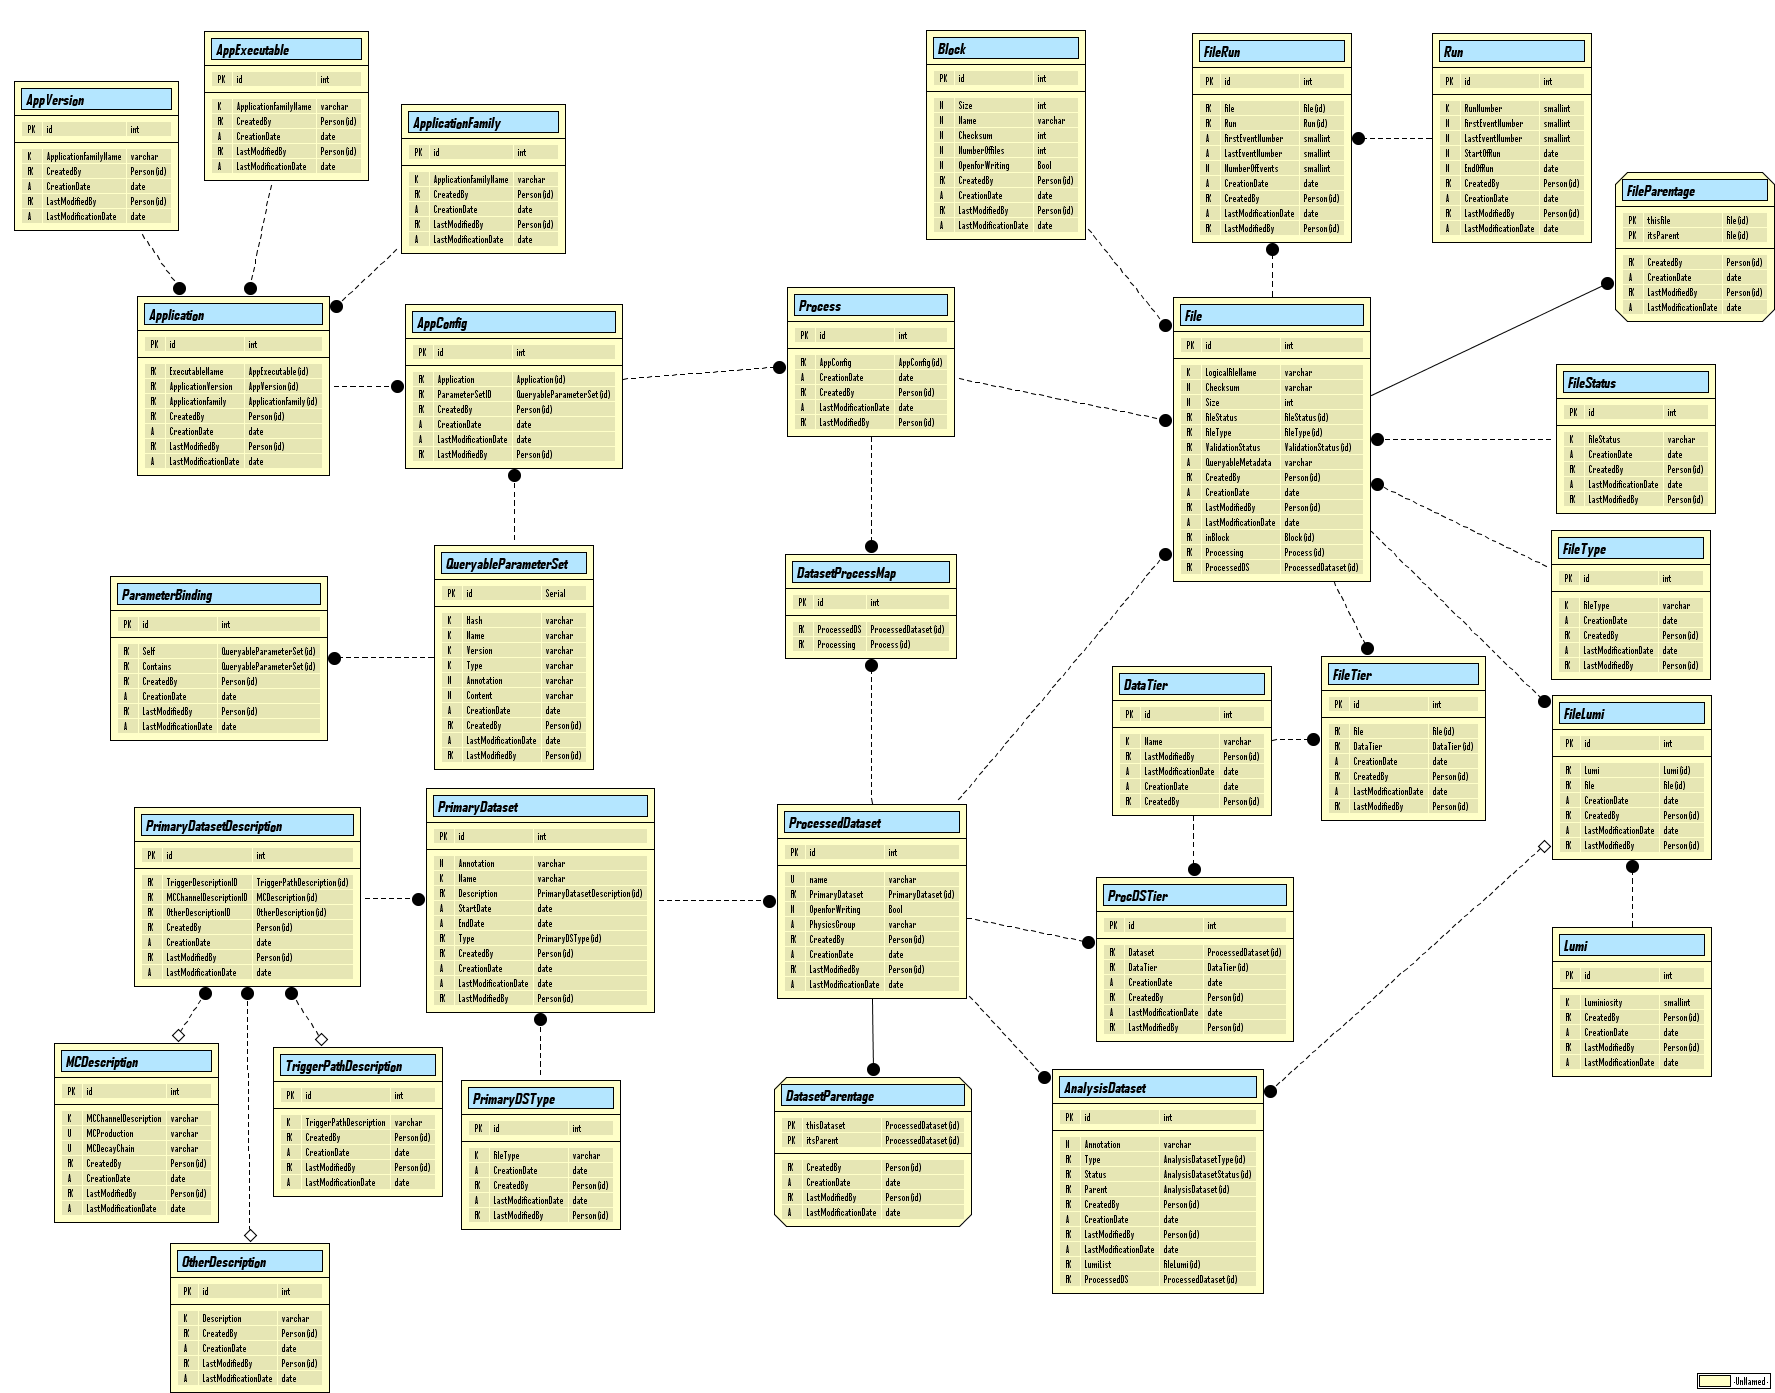
\includegraphics{figure/schema_07272006.eps}}
    \caption{New DBS schema design.}
    \label{fig:new-dbs-schema-design}
  \end{center}
\end{figure} 


\begin{enumerate}
\item{File}
 A File can contain multiple runs. A run can contain multiple files. The
 event range in a file represents the lowest bound event number to the
 highest bound event number. For example in a run r with a File f has
 event range 19,130. This does not imply that all the events are
 contiguous . There might be some events that can be missing. For example
 in this file f , only events 19,20,25,130 are present and rest of then
 are bad or missing.
 
 \item{FileRun}
 This table will represent many to many relationship in file and run.
 Note that the event range is an attribute of the FileRun table and not
 just of the File Table. This is required when multiple files will be
 merged into one single file. Then a File can spawn multiple runs and can
 spawn multiple event ranges. To discover all the event in this file we
 need to make event range an attribute of FileRun table. For example say
 a file f1 in run r1 contains events 3,16 and file f2 in run r2 contains
 events 5,15 and file f3 in run r1 contains events 2,13 . After we
 can merge f1,f2 and f3 into a big file ff, now FileRun table would
 contain two entries for file ff and run r1 and run r2. First entry for
 ff,r1 would have event range 2,16 and another entry for ff,r2 would
 contain 5,15. Note that of the files to be merged are in the same run
 then the event range would be minimum of lower bounds to maximum of
 higher bounds min(3,2),max(16,13).
 
 \item{FileParentage}
 This represents the lineage of the file. All the parents of the file are
 represented in this table. This file parentage is required at the file
 granularity. If it is not presents at this granularity , then there
 would be no way to correctly determining the exact parent of any
 particular file. Please note that this parentage is also specified at
 the ProcessedDataset level. The only reason for that is the optimization
 for discovery. One can easily find the parents of a dataset via
 traversing all the files and finding the parents of those files and then
 locating the datasets those files exists in. To optimize this discovery
 we need parentage at the dataset level too.
 
\item{ Block}
 This entity is entirely a concept of size and number of files. It can
 contain many files but if the collective size of those files reaches a
 certain limit (can be set by DBS admins), then it cannot accommodate any
 more files in it. In that case a block can be closed and a new block can
 be opened for adding new files into it. A block can be uniquely
 determined by its name that can also include dataset path along with its
 id.

(Dan's comments)
As was pointed out to me at the workshop, a block is supposed to
be homogeneous--all the contents should of a block should be of
the same data tier and processed data set.  This is important for
PhEDEx and for some of the management data discovery use cases we
discussed at last Friday's meeting.  PhEDEx in particular needs to
be able to efficiently find all the blocks for a given data tier
and processed data set, so this constraint may need to appear in
the schema as an optimization.
 
 \item{Lumi}
 A file can contains many Lumi Sections and a Lumi Sections can be
 contained in many files. These Lumi Sections are used for describing an
 analysis dataset which is conceptually more or less not related with
 files.

(Dan's comments) Missing here is what a luminosity section is.  The definition can be
found on this page:

https://twiki.cern.ch/twiki/bin/view/CMS/CMSTORTagonline

What's relevant for the DBS is that a luminosity section maps
onto a (contiguous) set of events defined at the time the data
are taken.  Since the the luminosity section boundaries are
defined by the DAQ, they will never change.  Luminosity sections
are not supposed to cross file boundaries--when the framework
splits a file for size limit reasons, it is supposed to do so
at a luminosity section boundary (I don't believe this is
implemented yet).

\item{DataTier}
 DataTier is infact related with the AppConfig via ParameterSet. But we
 need DataTier linked with Files also , since a physicists would require
 to know all the file in a dataset which has a certain DataTier. If
 DataTier would just be an ProcessedDataset Attribute, then the above
 query could not be executed. This is because a ProcessedDataset can
 spawn multiple DataTiers. If there is a restriction that a
 ProcessedDataset would only have a single DataTier then we would not
 required DataTier linkage with files at all. Also a File can have
 multiple DataTiers also, that is why all the more reasons to link
 DataTier with File. Note that FileTier is enough for associating and
 determining the DataTier with in a file as well as within a
 ProcessedDataset. So why would we need linkage of DataTier with a
 ProcessedDataset. The reason is same as that of File Parentage and
 ProcessedDataset Parentage. This is just an optimization for determining
 the DataTier with in a DataSet. One has to traverse all the files
 otherwise to know the DataTiers.

(Dan's comments)

As you note, a single AppConfig can write multiple files of different
data tiers at the same time, so the AppConfig <-> data tier
relationship is ambiguous.  The new definition of data tier is that a
data tier comprises a list of objects defined by a release which are
written to files of that tier.  The objects written to a file of a
given data tier will be defined by a release-dependent configuration
fragment, so what objects go into an AOD or RECO file may vary from
release to release.  I don't know how practical it will be to retrieve
these lists from the full ParameterSet -- it may be desirable to have
a separate table mapping (data tier, release) to a list of objects.
 
 \item{PrimaryDataset}
 PrimaryDataset is a placeholder for any type of data like raw or
 production. It is determined by the name and the description. Now this
 description can be of 3 different types: Monte Carlo type, Trigger Path
 type or some Generic Description. Therefore there are 3 tables
 representing each one. PrimaryDataset can contains raw data which means
 that it was not processed. To manage this within the schema, one can
 create a dummy ProcessedDataset with no link to any Application
 (AppConfig in this case). All the raw files can now be placed in this
 dummy ProcessedDataset

(Dan's comments)

There's actually two kinds of raw data: DAQ-RAW is the raw response
data from the detector in FED format, which is input to the HLT; RAW
is the output of the HLT.  Normally what will be injected into the DBS
is RAW data from the HLT, and the HLT is a cmsRun application with a
standard parameter set, so the normal RAW data will have real
processed data sets, not a dummy one.

 
 \item{Application}
 Application is uniquely determined by the Application Version,
 Application Executable and Application Family. There are three table
 representing each one and collectively they represents an Application
 \item{ParameterSet}
 ParameterSet is a collection of Parameters which are used to make a
 process. An entry in the ParameterSet can represent a single parameter
 or a composite parameter. For example a single parameter would contain
 name, value ,type and hash and a composite parameter would contain
 name, value ,type and hash  with or without content. Also a composite
 parameter would contain lot of other single or composite parameters.
 This is represented by the ParameterBinding table. One can look at these
 as a hierarchical directory structure. A single parameter would be
 lowest level directory which does not contain any other directory. A
 composite parameter would be a directory that may or may not contain
 other directory and may or may not contain a file (content). Hash
 uniquely identifies a parameter (both single and composite)
 
(Dan's comments)

I believe there's a way of getting the framework's pset parser to
give access to its internal parse tree, which could be used to
construct the QueryableParameterSet.  Parameter set's can have
fairly complicated nesting, so I'm a little worried about what a
query on this will look like, but I guess this is a reasonable
starting point.

 \item{AppConfig}
 A unique combination of an Application and a ParameterSet would
 represent an AppConfig. A file will be produced by a single AppConfig.
 That is why we have many to one relationship between AppConfig and File
 table. Note that a File has a relationship with ProcessedDataset, but
 that is not enough to determine the exact AppConfig used to produce the
 file. The reason being that a ProcessedDataset can spawn multiple
 AppConfig.
 
(Dan's comments)

While this is true, keep in mind that the framework can now merge
files with different provenance (the "fruit salad" mode), so different
objects in a single file may have different parentage/processing
history.

\item{ ProcessedDataset}
 Is uniquely represented by the PrimaryDataset , AppConfig and the input
 ProcessedDataset if any. Also, a ProcessedDataset can contain various
 AppConfig (Different version of Application). This satusfy the use case
 of creating many files with same application but different version of
 the software used. It can contain multiple files and therefore has
 one to may relationship with file. Also it can contain multiple DataTier
 which itself can spawn multiple ProcessedDataset and therefore many to
 many relationship among them. The reason for this linkage is for
 optimization purposes only and is described in FileTier section
 
 \item{AnalysisDataset}
 It is uniquely determined by Lumi Sections and ProcessedDataset. An
 AnalysisDataset is a subset of ProcessedDataset. From one
 ProcessedDataset many AnalysisDataset can be derived. Driving a new
 AnalysisDataset from an existing AnalysisDataset would mean to create a
 new ProcessedDataset. So essentially it will be a new AnalysisDataset
 from a ProcessedDataset again. Also AnalysisDataset can contain many
 Lumi Sections and same Lumi Sections can spawn multiple AnalysisDataset.
 Therefore we have AnalysisDSLumi table which represents many to many
 relationship among these entities.

(Dan's comments)

Analysis data set is more complicated than this.  The definition we've
been using is "a list of luminosity sections which were specified by
running an analysis query on a processed dataset at a particular
instant of time".  A processed data set may contain multiple instances
of a luminosity section processed with different application
configurations, so an analysis data set is determined by a processed
data set, a list of luminosity sections, and an AppConfig for each
luminosity section.

We haven't discussed how (or if) this maps onto MC data.
\end{enumerate}
\section{Client API}
\subsection{CSA06}
Python based (2.4.x and backward).
No external dependencies.
Independent of server implementation.
Exchange Python objects and Python data types with client(s).
Defines Client Data Structures/Types (CDS) for convenience (Derived from Python dictionary). CDS implement strict type checking for good reasons.
Throws DbsApiException.
Currently covers CRAB and Prod. Use-cases. Analysis use-cases are targeted during DM/DBS workshop at Cornell in July. 
Some dataset discovery APIs are also present, though we are in stone-age of dataset discovery. 
http://cmsdoc.cern.ch/~sekhri/Html/mc.htm
API Documentation at,

https://uimon.cern.ch/twiki/bin/view/CMS/CMS-DMS-DBS-API

Currently two type of interactions with DBS, 
Update DBS: The key is to understand the insert work flow for each type of information you need to record in DBS. Always a set of API calls in right order will work.
You need to know quite well what you want to do with DBS. Some advanced operations (Merge/Import/Export) need in-depth knowledge of DBS-API, DBS-Workflow and Dataset organization in DBS.
FWRK and DBS do not map 1-1 when it comes to Dataset organization. (not here!).
Example: you cannot insert a File Block, before you have inserted Primary Dataset and Processing.
DBS API is low level API, and calls for an interface layer between client Application(s), like ProdAgent, and DBS for a real work. One example is ProdAgent DBSInterface,
https://uimon.cern.ch/twiki/bin/view/CMS/ProdAgentDBSInterface

Simple use cases are coded in DBS Test cases (part of DBS API code).
Query DBS: Straight forward, you only need to understand ��CDS��, and how they relate to each other. Exposed via above mentioned web-tool.

\subsubsection{The API Structures (Python Implementation)}

Following describes the way dbsAPI Client data types look like schematically.
\begin{verbatim}
DbsPrimaryDataset:
      datasetName (name of primary dataset)

DbsApplication:
      executable 
      version
      family

DbsParameterSet:
      hash
      content

DbsApplicationConfig:
      application
      parameterSet

DbsProcessing:
      parent
      primaryDataset
      processingName
      applicationConfig
      isOpen

DbsProcessedDataset:
      primaryDataset
      processing
      datasetName
      dataTier
      datasetPath
      isDatasetOpen

DbsParent:
      parent
      type

DbsBlock:
      blockName
      processing
      blockStatusName
      numberOfBytes
      numberOfFiles
      fileList
      eventCollectionList

DbsFile:
      logicalFileName
      guid
      checkSum
      fileType
      fileStatus
      fileSize
      block

DbsEventCollection:
      collectionName
      numberOfEvents
      collectionStatus
      datasetPathName
      parentageList
      fileList


Python representation of Client Data Types

We have been working on coming up with a generic dictionary type representation for these types.

For example, a client data type can look like below,

class DbsBase(dict):
     """ Base Class for all DBS Client Data Types """
     def __init__(self, **args):
           dict.__init__(self)


class  DbsProcessedDataset(DbsBase):
   """ 
   Class for ProcessedDataset
   """
   def __init__(self, **args):
      DbsBase.__init__(self)
      self.setDefault("primaryDataset", None)
      self.setDefault("processing", None)
      self.setDefault("datasetName", None)
      self.setDefault("dataTier", None)
      self.setDefault("datasetPath", None)
      self.setDefault("isDatasetOpen", None)
      self.update(args)

class  DbsFile(DbsBase):
   """ 
   Class for File
   """
   def __init__(self, **args):
      DbsBase.__init__(self)
      self.setDefault("logicalFileName", None)
      self.setDefault("guid", None)
      self.setDefault("checkSum", None)
      self.setDefault("fileType", None)
      self.setDefault("fileStatus", None)
      self.setDefault("fileSize", None)
      self.setDefault("block", None)
      self.update(args)

\end{verbatim}

\subsubsection{The API Calls (Python implementation)}
The API will allow the argument for datasetPath to be a string, 
or polymorphicly an object. The string is convenient for users 
entering arguments by hand say, but the object is more convenient when 
using the result returned from another call.   
\begin{verbatim}
[] listDatasets(self, pattern="*"):
\end{verbatim}
   Given a string pattern, provide a list of DbsProcessedDataset objects by name.  The pattern option does not need to have 
three *'s (like */*/*). Returns always a list. If there are none, the 
return will be an empty list.

\begin{verbatim}
[] getDatasetContents(self, (string/obj) datasetPathName)
\end{verbatim}
   (This call is still being discussed with the CRAB developers.) Given a datasetPathName object, or string, return a list of file blocks and event collections. The search proceeds  via the tables processed\_datasets $\Rightarrow$ event\_collection $\Rightarrow$ file $\Rightarrow$ block. 

%************ This call is open for discussion ************
\begin{verbatim}
[] getDatasetBlockContents(self, (string/obj) datasetPathName, (obj) block):
\end{verbatim}
  (This call is still being discussed with the  CRAB developers.) Given a datasetPathName object, or string, and a block object name, returns all files and all parentage information. 
%***********************************************
\begin{verbatim}
?? getDatasetProvenance(self, (string/obj) datasetPathName, dataTierList=[]):
\end{verbatim}
(This call is still being discussed with the  CRAB developers. We need to understand how the provenance is described.)
\begin{verbatim}
   primaryDataset createPrimaryDataset(self, (obj) primaryDataset):
\end{verbatim}
Create a primary dataset and return the same primary dataset back. If
passed an object with the ID already set it will ignore it. 
The authorative source of the PrimaryDataset object ID is always the database.

\begin{verbatim}
   processing createProcessing(self, (obj) processing):
\end{verbatim}
Create a processing and return the same processing back. If
passed an object with the ID already set it will ignore it. 
The authorative source of the object ID is always the database.
\begin{verbatim}
   processedDataset createProcessedDataset(self, (obj) processedDataset): 
\end{verbatim}
Create a processed dataset and return the same processed dataset back. If
passed an object with the ID already set it will ignore it. 
The authoritative source of the object ID is always the database.
What is the significance of "name" for the processed dataset.

\begin{verbatim}
def createFileBlock(self, (obj) block): Refer to processing.
\end{verbatim}
\begin{verbatim}
   processedDataset createProcessedDataset(self, (obj) processedDataset):
\end{verbatim}
   Create a processed dataset with 0 size and 0 files in the block.
\begin{verbatim}
def insertFiles(self, block (defined by processing), fileList):
\end{verbatim}   
Insert the file or files in fileList into the specified block. The number of Files and total size for the block is adjusted accordingly. The table t\_block is locked  when files are being inserted.
\begin{verbatim}
def insertEventCollections(self, (string/obj) datasetPathName, eventCollectionList):
\end{verbatim}
   Remove the rule that EvColls must have Files.
   Remove the other rules about EvColl.
   So each EvColl has a list of "Parent" of object
   With a "type" like PU/Digi etc. Type of parent.
   Parent points to an EvColl.
   Parent EvColl points to parent dataset for parent evcoll.
   EvColl has list of LFN and they go into evcoll\_file table.
   Array inserts, 03 database inserts.
   Go one level parentage.
   Parents MUST already exist.
\begin{verbatim}
  block (list of files) getDatasetFileBlocks(self, (string/obj) datasetPathName):      
\end{verbatim}
Get a list of file blocks. Proceed  via processing $\Rightarrow$ block $\Rightarrow$ files. This call returns empty blocks as well if there are no files in them. This is something PheDEX will need to know. When a file is given to PheDEX 
it needs to know what block it belongs to. 
\begin{verbatim}
[] listPrimaryDatasets(self, (string) pattern="*"):
\end{verbatim}
\begin{verbatim}
[] listProcessedDatasets(self, (string) pattern="*"):
\end{verbatim}
\begin{verbatim}
[] listParameterSets(self, (string) pattern="*"):
\end{verbatim}   parameterSet contents matching, part of contents.
\begin{verbatim}
[] listApplications(self, (string) pattern="*"):
\end{verbatim}
\begin{verbatim}
  pattern= /family/executable/version
\end{verbatim}
\begin{verbatim}
[] listApplicationConfigs(self, (string) pattern="*"):
\end{verbatim}
   pattern=applicationName
>
Consider the usecase of trying to narrow down from a primary dataset,
to a particular tier, to an analysis dataset.  We are missing the 
ability to list dataset tiers, need the call 
\begin{verbatim}
[] listDatasetTiers(self, (string) pattern="*")
\end{verbatim}
The argument could be like /primaryDataset/DataTier, or just DataTier
\begin{verbatim}
[] listFileBlocks(self, datasetPathName):
\end{verbatim}

\begin{verbatim}
def closeFileBlock(self, block):
\end{verbatim}
The block must have an object.
(?BlockName: Processing\#BlockID)




\subsection{Extensions and Changes for next generation DBS}
\section{Plan of Work}
A time table for the DBS work is shown in Table~\ref{tab:dbs-work-plan}.
\begin{table}[htb]
    \caption{DBS workplan for the Aug. 2006 through Jan 2007 in detail, rough plan beyond. to July 2007.  }
    \label{tab:dbs-work-plan}
    \begin{center}
      \begin{tabular}{|l|p{1.5in}|p{1.5in}|p{1.5in}|} \hline 
Date & CSA06 DBS & 2nd Gen. DBS & Comments \\ \hline
Aug. 2006 & Updates to API, minimal updates to schema, operation of existing service. Initial discover tools for MC production & Roadmap development  &    \\ \hline
Sep. 2006 & Operations, global and local relationship field experience.   & Use case development, API and schema review and revisions.  &    \\ \hline
Oct. 2006 & Maintanence    & Schema, API prototyping. Test development.Discovery tools & \\ \hline
Nov. 2006 & Migration plan   & Transfer tools CSA to 2G., Production server planning  &    \\ \hline
Dec. 2006 &     &   &    \\ \hline
Jan. 2007 &    &   &    \\ \hline
Feb.-Jul. 2007 &    &   &    \\ \hline
      \end{tabular}
    \end{center}
  \end{table}  
\pagebreak
\begin{thebibliography}{9}
  \bibitem {dls-twiki} {DLS twiki: https://twiki.cern.ch/twiki/bin/view/CMS/DLS}
  \bibitem{CTDR} {\bf ????}, , {\bf CMS Computing Technical Design Report}
  \bibitem {bogus} {all items below are bogus}
  \bibitem {smtp} {Simple Network Management Protocal}
  \bibitem {mrtg} {Multi Router Traffic Grapher}
  \bibitem {pool-ral} {POOL-RAL: POOL Persistence Framework, url{http://pool.cern.ch/ .}
  \bibitem {frontier}{FroNTier Project, see S. Kosyakov, et. al.,''Frontier: High Performance Database Access Using Standard Web Components,'' Proceedings of the CHEP\,04 Conference, Interlaken Switzerland, 27 September - 1 October, 2004,
Available at http://lynx.fnal.gov/ntier\-wiki/Additional\_20Documentation.}
  \bibitem {tomcat}{Tomcat home page: http://tomcat.apache.org}
  \bibitem {squid}{D. Wessels, Squid: The Definitive Guide, O'Reilly and Associates, 2004. Squid home page: http://www.squid-cache.org.}
  \bibitem {squid-accel-mode}{op. cite~\cite{squid}, pp. 302-314.}}
%last } is a mystry but latex asked for it. 
  \bibitem {squid-objects}{For additional information see http://lynx.fnal.gov/ntier-wiki/Squid\_20performance\_20for\_20big\_20objects}
  \bibitem{CherryPy} {\it http://www.cherrypy.org}
  \bibitem{Cheetah} {\it http://www.cheetahtemplate.org}
  \bibitem{SQLAlchemy} {\it http://www.sqlalchemy.org}
\end{thebibliography}

\pagebreak



\end{document}
